Figure~\ref{fig:4:fw} in Chapter~\ref{chap:cc.fw} shows the structure of the
congestion control framework described in this thesis. The framework
categorizes \emph{In-path} sources and \emph{out-of-band} signaling for
implementing congestion control, which are discussed in this chapter. This
chapter is based on our work on Multipath RTP (MPRTP), which is documented in
\citepub{c:mprtp}, in \cite{draft.mprtp}, \cite{draft.mprtp.sdp},
\cite{Globisch:AsymGrpComm}, and \cite{draft.rtcp.overlay}.

In \citepub{c:mprtp}, we propose the following: design goals of implement a
multipath protocol for multimedia, protocol details, scheduling algorithm to
send media packets over multiple paths, a dejitter buffer implementation to
playout packets smoothly even when the path skew is high. We evaluate the
performance of the proposed mechanisms in diverse scenarios in our testbed.
Lastly, we discuss the system consideration for deployment.

\section{Multipath RTP (MPRTP)}

The Internet backbone has evolved over the past decades to a mesh of service
providers with manifold peerings that are generally capable of offering a
number of (independent) paths between two nodes. Networks often use multiple
attachment points for resilience purposes, such as data enterprise networks or
data centers and even routers for SOHO networks support multiple access
networks~\cite{draft.fun.multi, draft.homenet.arch}. Additionally, many hosts
today feature multiple network interfaces (e.g., WLAN and 3G on mobile
devices), this may yield the possibility for two endpoints to communicate via
multiple paths. While exploiting multipath characteristics
\cite{Wischik:2008:RPP} has been explored for TCP (e.g.,
MPTCP)~\cite{rfc6824}, the requirements for real-time traffic differs notably
and TCP can only serve real-time communication within tight constraints of
network characteristics~\cite{Brosh:tcp-real-time}. In the multipath case, the
scheduling algorithms do not consider real-time bounds when spreading data
segments across different paths and diverse paths may lead to worst case delay
and thus even longer buffering time.

\begin{figure}
\centerline {
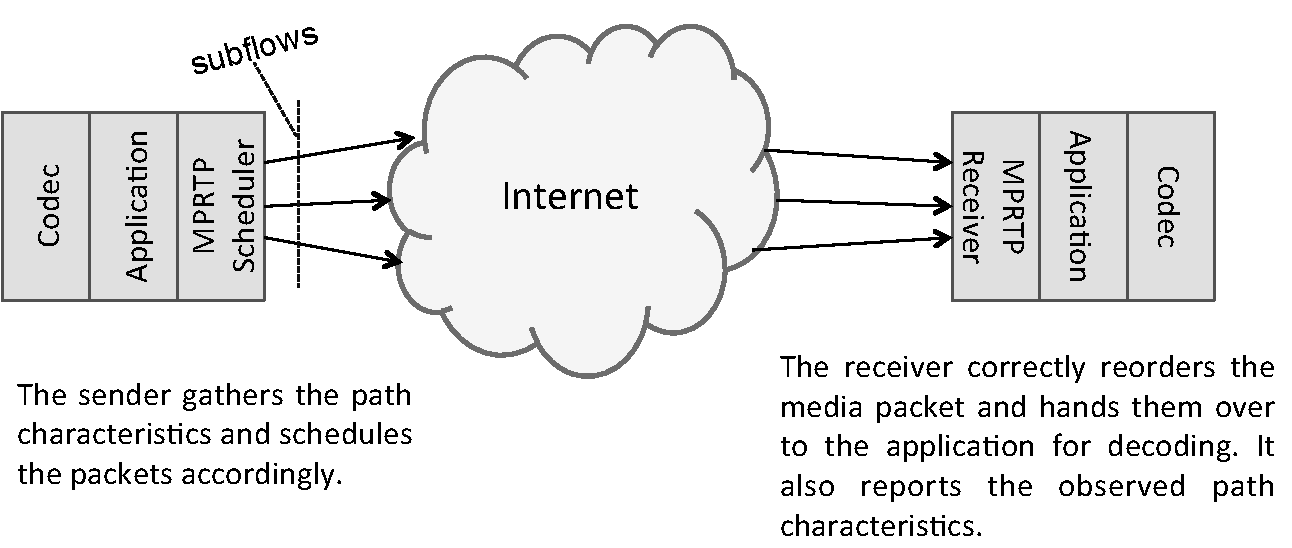
\includegraphics[width=0.9\textwidth]{chap7-fig_mprtp-1}
}
\caption{System Overview: A sender uses multiple paths to stream media
  to a receiver.  The receiver uses a dejitter buffer to reorder
  packets and sends per-path characteristics to the sender that
  distributes the packets based on the reported values.}
\label{chap7:fig_mprtp}
\end{figure}

We propose Multipath RTP (MPRTP) as a backwards compatible extension to
RTP~\cite{rfc3550}, it is documented in \cite{draft.mprtp} and defines the
basic mechanisms to operate across multiple parallel paths.
Figure~\ref{chap7:fig_mprtp} shows a macroscopic system overview of MPRTP. The
primary use-case for MPRTP is transporting media flows between multi-homed
endpoints. Such endpoints could be residential IPTV or telepresence devices
that connect to the Internet through two different Internet service providers
(ISPs), or mobile devices that connect to the Internet through 3G and WLAN
interfaces. By allowing RTP to use multiple paths for transmission, the
following gains can be achieved:

\begin{enumerate}
\setlength{\itemsep}{5pt}

\item \textbf{\texttt{Higher quality}}: Pooling the resource capacity of
multiple Internet paths allows higher bit-rate and higher quality codecs to be
used. From the application perspective, the available bandwidth between the
two endpoints increases.

\item \textbf{\texttt{Load balancing}}: Transmitting an RTP stream over
multiple paths reduces the bandwidth usage on a single path, which in turn
reduces the impact of the media stream on other traffic on that path. Also by
seamlessly offloading a flow from one path to another allows for some gains,
for example, reduces energy consumption, reduces access costs, or reduces
network latency.

\item \textbf{\texttt{Fault tolerance}}: Using multiple paths in conjunction
with redundancy mechanisms (FEC, re-transmissions, etc.), outages on one path
have less impact on the overall perceived quality of the stream. This can also
enable seamless handover in the case of mobility, i.e., moving from one
network to another.

\end{enumerate}


\begin{figure}
\centerline {
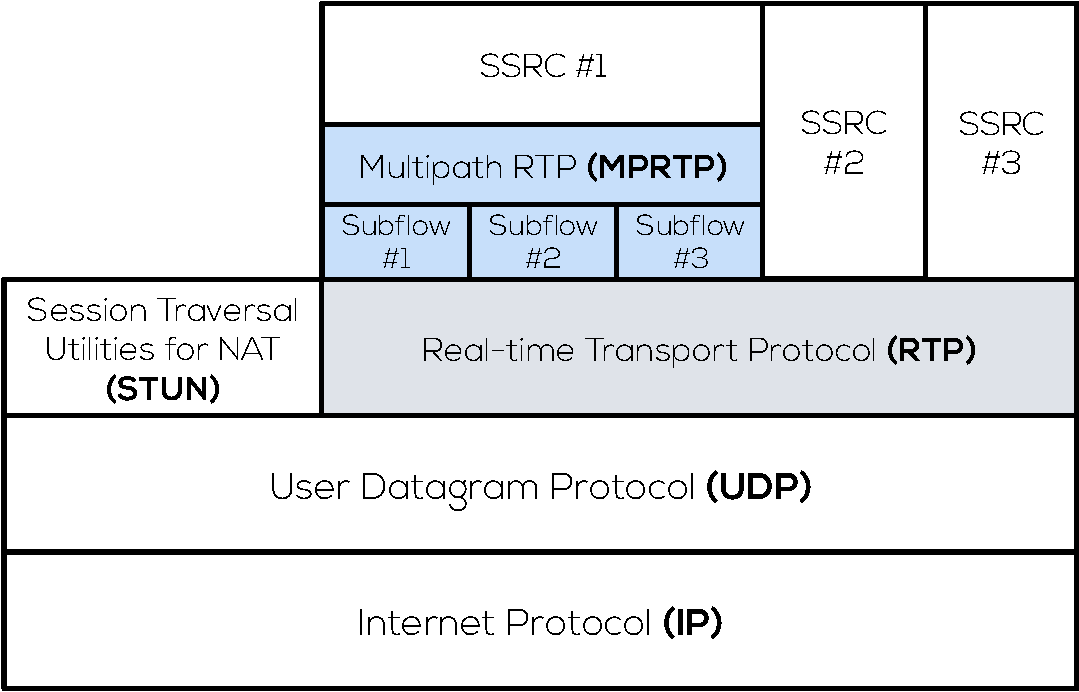
\includegraphics[width=0.75\textwidth]{chap7-fig-mprtp-stack}
}
\caption{Visualizing the RTP and MPRTP communication stack, SSRC$\#1$ uses
MPRTP while SSRC$\#2$ and SSRC$\#3$ uses single path RTP.}
\label{chap7:fig_mprtp_arch}
\end{figure}

Figure~\ref{chap7:fig_mprtp_arch} compares the network stack of a single path
and a multipath-capable endpoints. SSRCs\#2 and SSRC\#3 use a single path,
while SSRC\#1 uses multiple paths (with two subflows for the two paths).

The design goals for MPRTP from our perspective are: MPRTP-enabled system to
be able to make use of multiple paths and adapt to their relative capacity
changes by redistributing the load. As different paths will likely exhibit
different RTTs, mechanisms must be developed to overcome the resulting skew.
Furthermore, the choice of suitable transmission paths should reflect the
demands of the application. From a protocol perspective, RTP must be extended
to perform these functions, yet maintain backwards compatibility. 

\section{Call Establishment and NAT Traversal}

When endpoints want to use multiple paths or offload traffic onto another path
(or interface) or move between networks, it requires the endpoint to either
change its IP address or use multiple IP addresses at the same time.
Typically, an endpoint changing its IP addresses breaks some of the higher
level protocols (e.g., TCP, RTP), unless the higher level protocol is designed
to be oblivious to the changes in IP address (e.g., SCTP~\cite{rfc4960}).

Various techniques exist for handling mobility, such as, Mobile IP, Proxy
Mobile IP, Locator/ID Separation Protocol (LISP), but these techniques are not
useful for enabling multipath because they attempt to assign a static IP
address to the endpoint and hence disables the use of multiple paths.
Endpoints will generally use a signaling protocol to establish a media
session. With the existence of such a signaling relationship, two alternatives
become available to advertise an endpoint's multiple interfaces:
\emph{in-band} (over the media path) or \emph{out-of-band} (over the signaling
path).

Typically, performing interface advertisement is tightly coupled with NAT and
firewall traversal. Endpoints implement NAT and FW traversal using Interactive
Connectivity Establishment (ICE)~\cite{rfc5245} procedures, which enables the
endpoints to ascertain connectivity between the endpoints by performing
connectivity tests before transmitting media. The endpoint usually advertises
the multiple interfaces in SDP, which usually couples the interface
advertisement to the offer/answer mechanism. The offer/answer mechanism is
excessive in this case, because a declarative mechanism would suffice. The
endpoint mainly wants to notify the other endpoints of its multiple
interfaces. Likewise, when multiple interfaces become available at the other
endpoint, it would notify its peers.

To summarize, in \cite{draft.mprtp}, we define an \emph{in-band} mechanism to
advertise interfaces in RTCP. The endpoint is able to update its existing
interfaces or advertise new ones, whenever the RTCP interval expires.
Advertising in-band is mainly useful when the endpoints are not deployed
behind NATs or the ICE agent works together with the MPRTP
stack~\cite{draft.mice}. In \cite{draft.mprtp.sdp}, we define the \emph{out-of
band} mechanism in SDP. The endpoint in this case performs the first round of
offer/answer exactly like it would do for a multimedia session using a single
path, but indicating it supports MPRTP and containing multiple \emph{ICE
candidates}. Later, when the connectivity checks for more than one path are
successful, each endpoint advertises its MPRTP interfaces.
Figure~\ref{chap7:fig_mprtp_arch} show the interworking of the MPRTP stack
with an ICE Agent implementing STUN connectivity checks. In \citepub{c:mprtp}
we show that advertising the multipath interfaces \emph{in-band} leads to a quicker call establishment than when advertising \emph{out-of-band}.


\section{Offloading and Multihoming}

In \citepub{c:mprtp}, we focus on spreading a constant bit rate (CBR) media
stream across multiple paths, for which we present a scheduling algorithm for
allocating traffic based on path characteristics. We use an adaptive dejitter
buffer at the receiver so that the endpoint can playback media packets from
paths with diverse characteristics. However, our work is orthogonal to rate
adaptation--which would just change the total media rate to spread across each
subflow.


\begin{figure}
    \centerline{
        {\includegraphics[width=0.8\textwidth] %clip=true, trim=0 1cm 0 1.5cm]
        {chap7-graph_variable_bw_13073-2p5-2}}
    }
    \caption{MPRTP offloading from a constrained path.}
    \label{chap7:fig_sim_var_bw}
\end{figure}

\textbf{\texttt{Offloading}}: In this scenario, the e2e capacity on one path
is variable, it demonstrates the sensitivity of the scheduling algorithm to
the changes in network capacity, which may be caused by \emph{cross-traffic}.
Path B in Figure~\ref{chap7:fig_sim_var_bw} shows the link with variable e2e
capacity and the per-instant bandwidth utilization by an MPRTP subflow. Note
that the scheduling algorithm uses cues on one path to reallocate the media on
to the other paths (observe the points where the link rate drops). The
scheduling algorithm also tries to probe the network, so that an equilibrium
state of fair sharing can be achieved. However, this is done at long
time-scales (order of seconds) so that the per-path load does not oscillate.

\begin{table}[!t]%htbp]
\centering
% \resizebox{\textwidth}{!}{%\scalebox{0.75}
{
\begin{tabular}{ccccc} \hline
Path Characteristic & Avg. PSNR & $\sigma_{PSNR}$ & PLR\\ \hline
Offloading & 42.93 & 2.23 & 0.772 \\
Multihoming & 46.7173 & 0.21 & 0.33 \\ \hline
\end{tabular}
}
\caption{Performance of multipath scheduling when offloading (from a
constrained path) and multihoming (with WLAN and 3G paths)}
\label{table-bb-3g}
\end{table}

\textbf{\texttt{Multihoming}}: Figure~\ref{chap7:fig_sim_bb_3g} shows the
bandwidth utilization of a WLAN and 3G path and the overall bandwidth
distribution between the paths. The bandwidth is more evenly shared except
when the 3G path is constrained, the scheduling algorithm offloads the
remaining media on to the WLAN path, however, it does not quickly reallocate
the bandwidth it took away from the link to avoid bandwidth oscillations. This
is a useful feature for the scheduling algorithm because it can then use the
passive or idle paths for fallback. Moreover, the 3G path encounters packet
losses more often than on the WLAN path, which makes the scheduling algorithm
prefer sending more media over the WLAN path. Despite using two lossy paths
the PSNR of the media stream (see Table~\ref{table-bb-3g}) in this scenario is
close to optimum.

\begin{figure}
    \centerline{
        {\includegraphics[width=0.8\textwidth] %clip=true, trim=0 1cm 0 1.5cm]
        {chap7_graph_bb_3g_s17075-2p3-2}}
    }
    \caption{A multihomed endpoint load-balancing a media flow over WLAN and
    3G paths.}
    \label{chap7:fig_sim_bb_3g}
\end{figure}

% \textbf{Conclusions}: We have explored the criteria for assigning traffic
% shares as a function of the diverse path properties and presented
% considerations for scheduling algorithms. Our evaluation shows that our
% design 1) allows exploiting multiple paths without performance degradation
% compared to suitable single-path cases—so that it is safe to deploy—and 2)
% enables load distribution and capacity aggregation in diverse scenarios.
% Mobile users (and operators) may benefit from aggregating or dynamically
% shifting load between different wireless interfaces of their mobile devices
% and MPRTP may assist well in bundling multiple wireless access networks for
% vehicular Internet access.

\section{Applying MPRTP to Application Layer Multicast}


Various conference server architectures can be used to distribute the media in
a many-to-many communication scenario: centralized, unicast receive with
multicast send, full mesh, overlays, and trees
\cite{Li2010a,Noh2008,Singh2001}. When developing a conferencing server, the
scalability, reliability, quality and delay characteristics, for each of these
architecture needs to be considered. In group communication, we assume a low
peer churn i.e., all participants arrive and leave roughly at the same time.
The use of multiple Application Layer Multicast (ALM) trees for media delivery
minimizes the end-to-end delay and results in asymmetric relationships between
participants and introduces complex forwarding. Chu et al. show ALM as a
viable solution for real-time conferencing over the Internet~\cite{Chu2001}.
Banerjee et al.\cite{Banerjee2002} present an ALM protocol that has a
hierarchical control structure with low overhead. Noh et al.~\cite{Noh2008}
use multiple trees to reduce the end-to-end delay and determine the optimal
number of ALM trees depending on specific network characteristics. They
conclude that the fan-out of a peer influences the trade-off between the
propagation delay and the queuing delay. Li et al.~\cite{Li2010a} describes
the use of multiple trees as a mechanism to scale to more clients by
introducing multiple focus-mixer structures where each structure is dedicated
to serving a set of clients in a region.